\documentclass[a4paper,twoside,12pt]{report}
% Richard Klein (2020,2021)

% Include Packages
%\usepackage[a4paper,inner=3.5cm,outer=2.5cm,top=2.5cm,bottom=2.5cm]{geometry}  % Set page margins
\usepackage{fullpage}
\usepackage{float}                  % Allows 'Here and Only Here' [H] for Floats
\usepackage{url}                    % \url{} command
\usepackage{charter}                  % Set font to Times
\usepackage{graphicx}               % \includegraphics
\usepackage{subfigure}              % Allow subfigures
\usepackage{amsmath}
\usepackage{amssymb}
\usepackage{amsthm}
\usepackage{booktabs}
\usepackage{parskip}
\usepackage[all]{nowidow}
\setnoclub[2]
\setnowidow[2]

% Referencing
% Provides \Vref and \vref to indicate where a reference is.
\usepackage{varioref} 
% Hyperlinks references
\usepackage[bookmarks=true,bookmarksopen=true]{hyperref} 
% Provides \Cref, \cref, \Vref, \vref to include the type of reference: fig/eqn/tbl
\usepackage{cleveref} 
% Setup Hyperref
\hypersetup{
  colorlinks   = true,              %Colours links instead of ugly boxes
  urlcolor     = blue,              %Colour for external hyperlinks
  linkcolor    = blue,              %Colour of internal links
  citecolor    = blue                %Colour of citations
}
% Names for Clever Ref
\crefname{table}{table}{tables}
\Crefname{table}{Table}{Tables}
\crefname{figure}{figure}{figures}
\Crefname{figure}{Figure}{Figures}
\crefname{equation}{equation}{equations}
\Crefname{equation}{Equation}{Equations}

% Wits Citation Style
\usepackage{natbib} % Force natbib.sty to put citation labels in the reference list
\makeatletter
\renewcommand\NAT@biblabel[1]{\def\citeauthoryear##1##2{##1 ##2}[#1]\hfill}
\renewcommand\NAT@bibsetup[1]{%
  \setlength{\itemsep}{\bibsep}\setlength{\parsep}{\z@}}
\def\@lbibitem[#1]#2{%
  \if\relax\@extra@b@citeb\relax\else
    \@ifundefined{br@#2\@extra@b@citeb}{}{%
     \@namedef{br@#2}{\@nameuse{br@#2\@extra@b@citeb}}}\fi
   \@ifundefined{b@#2\@extra@b@citeb}{\def\NAT@num{}}{\NAT@parse{#2}}%
   \item[\hfil\hyper@natanchorstart{#2\@extra@b@citeb}\@biblabel{#1}%
    \hyper@natanchorend]%
    \NAT@ifcmd#1(@)(@)\@nil{#2}}
\makeatother


\bibliographystyle{named-wits}
\bibpunct{[}{]}{;}{a}{}{}  % to get correct punctuation for bibliography
\setlength{\skip\footins}{1.5cm}
\newcommand{\citets}[1]{\citeauthor{#1}'s \citeyearpar{#1}}
\renewcommand\bibname{References}  

\pagestyle{headings}

\pagestyle{plain}
\pagenumbering{roman}

\renewenvironment{abstract}{\ \vfill\begin{center}\textbf{Abstract}\end{center}\addcontentsline{toc}{section}{Abstract}}{\vfill\vfill\newpage}
\newenvironment{declaration}{\ \vfill\begin{center}\textbf{Declaration}\end{center}\addcontentsline{toc}{section}{Declaration}}{\vfill\vfill\newpage}
\newenvironment{acknowledgements}{\ \vfill\begin{center}\textbf{Acknowledgements}\end{center}\addcontentsline{toc}{section}{Acknowledgements}}{\vfill\vfill\newpage}

\begin{document}
\onecolumn
\thispagestyle{empty}

\setcounter{page}{0}
\addcontentsline{toc}{chapter}{Preface}
\ 
\begin{center}
  \vfill
  {
  \huge \bf \textsc{Title of Research}\\
  \large Subtitle\\[20pt]
  \large School of Computer Science \& Applied Mathematics\\
  \large University of the Witwatersrand\\[20pt]
  \normalsize
  Your Name\\
  Your Student Number\\[20pt]
  Supervised by Dr McProfessorFace\\[10pt]
  \today
  }

  \vfill
  \vfill
  
\includegraphics[width=1.5cm]{images/wits}
  \vspace{10pt}\\
  \small{Ethics Clearance Number: XX/XX/XX}\\[10pt]
  \small{A proposal submitted to the Faculty of Science, University of the Witwatersrand, Johannesburg,
in partial fulfilment of the requirements for the degree of Bachelor of Science with Honours}\\
\end{center}
\vfill
\newpage

\pagestyle{plain}
\setcounter{page}{1}

\phantomsection
\begin{abstract}
Abstract things....
\end{abstract}

\phantomsection
\begin{declaration}
I, ---------, hereby declare the contents of this research proposal to be my own work.
This proposal is submitted for the degree of Bachelor of Science with Honours in Computer Science at the University of the Witwatersrand.
This work has not been submitted to any other university, or for any other degree.
\end{declaration}

\phantomsection
\begin{acknowledgements}
Thanks World.
\end{acknowledgements}


\phantomsection
\addcontentsline{toc}{section}{Table of Contents}
\tableofcontents
\newpage
\phantomsection
\addcontentsline{toc}{section}{List of Figures}
\listoffigures
\newpage
\phantomsection
\addcontentsline{toc}{section}{List of Tables}
\listoftables
\newpage
\pagenumbering{arabic}


\chapter{Introduction}

\section{Hello World}

Introduction things...\\

\section{Another Section}

\subsection{This is a Subsection}

\subsubsection{This is a subsubsection}

This is just a paragraph

\subsection{A Subsection about Citation Style}

Citations are important. Citation style for Computer Science is:

\begin{itemize}
    \item When used in the text, use the authors with the date in brackets:\\ \citet{klein17} say very important things.
    \item When used as a reference after a face, put everything in brackets:\\ Import things are true \citep{klein17}.
\end{itemize}


\chapter{Background}
\label{background}

In this section, we discuss the prerequisite theory for the methods being used in this research. We start by briefly defining the reinforcement learning (RL) problem in Section \ref{mdp} and relate it to its foundational theory, the Markov Decision Process (MDP). In section \ref{drl} we discuss deep reinforcement learning, the core method of our research. As a supplement to future sections, we spend section \ref{cnn} discussing convolutional neural networks (CNN), an essential deep learning algorithm used for processing the images in our research environment. We also discuss the residual network, our specific CNN of choice in section \ref{resnet}. Finally in section \ref{policygrad} and \ref{contrastivelrn} we look at the two methods that we combine in this research for a novel enquiry, Proximal Policy Optimization (PPO) and a Simple Framework for Contrastive Learning of Visual Representations (SimCLR). 

\section{Reinforcement learning and Markov Decision Processes}
\label{mdp}

where $t$ is the time-step of our interaction and $\tau$ is the terminal or goal state that we wish to be in, defined as infinity for continuous tasks \citep{janner2019trust}. The variable $\gamma$ is the discount factor which varies depending on how much value we wish to place on future rewards. Determining the value of a policy requires that we either parameterize it using a function approximator, or determine state values using a value function \citep{moderndrl}. A value function is a numerical representation of how good it is for an agent to be in some state $s$ \citep{moderndrl}. It is typically equal to the value of the total reward that the agent can expect to receive being in a state and continuing to take actions within the MDP \citep{sutton_barto_2018}. 

Markov Decision Processes (MDP) are a classical formalisation of the RL problem which are essentially a series of decisions made in sequence with each action influencing the subsequent states and feedback signals. In this section we formulate the RL problem as an MDP using a series of mathematical expressions. We define returns, discount factors, value functions and Bellman equations. This forms the basis for all RL theory in this paper.


The RL problem consists of a cyclical interaction loop between two entities, the learner, hence referred to as the agent  and an external construct, hence referred to as the environment.

\begin{figure}[ht]
	\centering
	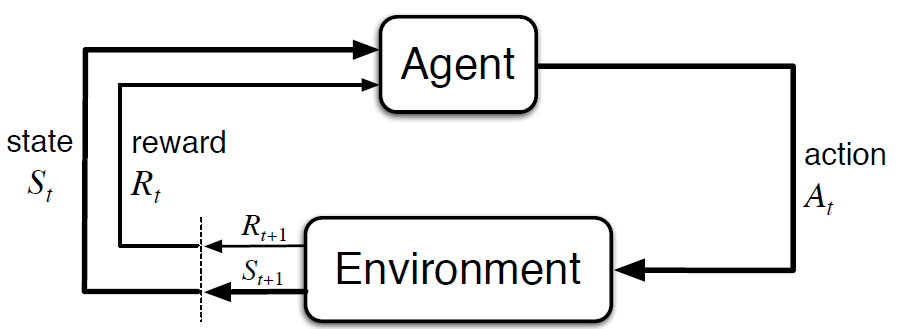
\includegraphics[width=0.7\linewidth]{images/mdprl.png}
	\caption{The interaction loop between the agent and environment. \citep{sutton_barto_2018}}
	\label{fig:mdprl}
\end{figure}

The Figure \ref{fig:mdprl} describes the interaction loop between these entities as a series of time steps. These steps can be discrete or continuous but for the purposes of our explanation we will use discrete time steps. At any given step $t$, the agent will find itself in a circumstance called a state $s$, where $s \in \mathcal{S}$, where $\mathcal{S}$ is a set of all states reachable within the environment. Within this circumstance it is allowed to take an action $a$, where $a \in \mathcal{A}(s)$, where $\mathcal{A}(s)$ is the set of all actions available in state $s$. In the subsequent timestep $t+1$, the agent will receive a numerical signal called a reward and a new state $s_{t+1}$. We refer to this reward as $r \in \mathcal{R}_{t+1} \subset \mathbb{R}$. These cyclical sequences of state, action and reward form what is referred to as a trajectory. 

For the purposes of this thesis, we limit our explanation of MDPs to finite MDPs. In a finite MDP, all $\mathcal{S}$, $\mathcal{A}$, $\mathcal{R}$ have a finite number of elements. $\mathcal{R}_t$ and $\mathcal{S}_t$ for any timestep $t$ have discrete probability distributions based only on the preceding state and action. This can be mathematically formulated by the following equation: 
\begin{equation}
\ p(s', r|s, a) \, \dot{\mathbf{=}} \, \textrm{Pr}\{\mathcal{S}_t=s', \mathcal{R}_t=r | \mathcal{S}_{t-1}=s, \mathcal{A}_{t-1}=a\}
\label{dynamics}
\end{equation}

The probability function $p$ defined in equation \ref{dynamics} defines the dynamics of the MDP and can be used to compute other information about the environment, such as, state-transition probabilities, the expected rewards for particular state-action pairs and state-action next-state triples. This information is initially unknown and is discovered through a continuous interaction loop with the environment illustrated in the figure \ref{fig:mdprl}. 

The goal or purpose of an RL agent is to maximize the numerical feedback signal or reward it is given, through taking actions in various states of the environment, at some time step. This goal must be maximised cumulatively over time, not just for immediate rewards, and the rewards must be representative of the correct action we want the agent to perform in its environment. For this we must understand what we want the agent to receive in a given environment, and then attach rewards to this environment so that the agent discovers how to achieve it in the best possible way through the duration of its interactions. This concept is known as the reward hypothesis, or, that a goal is the maximization of the expected value of the cumulative sum of the received numerical feedback signal.

We now formally define the goal of the agent as the cumulative expected return over a set of time steps. For a fixed number of time steps the set of states $S$ will contain a terminal state $\tau$. This is referred to as an episode. For a continuous task $\tau$ is infinity. We define the cumulative expected return as $G_t$. The agent performs its interaction loop receiving a reward $r$ at each successive time step $t$. The agent must take action within each state $s$ to optimize $G_t$ by generating the largest possible reward sequence before reaching $\tau$, or reach a maximum $G_t$ as fast as possible for a continuous task.  

To perform optimally, an agent must consider the value of a future rewards in comparison with its present reward.  

\subsection{Deep reinforcement learning}
\label{drl}

Deep reinforcement learning (DRL) methods can be split according to two basic approaches. The first are value-based methods which keep function approximated state-action values stored in order to determine an optimal policy. They keep no explicit representation of this policy as this can be inferred directly from state values. Instead, they try to assess $Q:S \times A \rightarrow R$ \citep{moderndrl}, or the value of each state-action combination. In contrast, policy gradient methods keep an explicit, parameterized representation of the policy that is updated from experience gained whilst learning. It uses this to determine the best action $a_t$ when in some state $s_t$, and instead tries to solve for $\pi : S \rightarrow A$ \citep{moderndrl}. 

\section{Policy gradient methods}
\label{policygrad} 
The modern implementation of deep reinforcement learning uses deep neural networks to parameterize the state-action values of value-based methods and the policies of policy gradient methods \citep{policygrad}. For policy gradient algorithms, the policy, defined as the probability of an agent taking action $a$ in an arbitrary state $s$, is augmented as follows $\pi_\theta(a|s;\theta)$. The optimization objective can be mathematically defined as follows:
\begin{align}
    J(\pi_\theta) = E_{\tau \sim \pi_\theta} [R(\tau)] = \int_{\tau} P(\tau,\theta)R(\tau) \\
    \theta_{k+1} = \theta_{k} + \alpha \nabla_{\theta}J(\pi_{\theta})|_{\theta_{k}}
\end{align}
Equation 2 structures our cost function as the expected rewards equal to the sum of all probabilities $P$, of a trajectory $\tau$ multiplied by its rewards $R(\tau)$. This this can be represented as the integral over $P(\tau,\theta)R(\tau)$. The objective of the policy gradient method is then to find a policy $\pi_\theta$ to generates some trajectory $\tau$, that maximises the function $J$. This is performed through the gradient ascent step detailed in equation 2.3. To compute the cost function or expected value in this algorithm, we need to use a form of the probability function that is easily differentiated and summed \citep{policygrad}. \medskip

Let us recount that the probability of a trajectory $P(\tau|\theta)$, due to the Markov property is $\rho_0 (s_0)\prod^{T}_{t=0} P(s_{t+1}|s_t,a_t)\pi_{\theta}(a_t,s_t)$ where $\rho$ is the sample distribution from which $s_0$ is drawn. The optimization uses a technique known as logarithmic differentiation to allow the algorithm to use back propagation on the parameters $\theta$ more simply. $T$ in this function can be defined as some terminal state or horizon. The partial derivative with respects to $\theta$ of $P(\tau|\theta)$ can be expressed as $\nabla_\theta P(\tau|\theta) = P(\tau|\theta)\nabla_\theta \: log \: P(\tau|\theta)$. The log representation allows us to take the sum of the probability of a trajectory $P(\tau|\theta)$ instead of its product, allowing for a more seamless gradient calculation. This is defined as  $log \: P(\tau|\theta) = \rho_0(s_0) + \sum^{T}_{t=0} log \: P(s_{t+1}|s_t,a_t) + log \: \pi_{\theta}(a_t,s_t)$. When taking the derivative with respect to $\theta$, the initial state and $log\: P(s_{t+1}|s_t,a_t)$ have no dependency on the $\theta$ variable, and hence their values will always be $0$. This also illustrates why we require the log form of the derivative, as using the normal representation of $P(\tau|\theta)$ would make gradient ascent impossible, as taking the product will always yield $0$ \citep{policygrad}. The final representation of the gradient ascent cost function will be:
\begin{align}
    \nabla_\theta J(\pi_\theta) = E_{\tau \sim \pi_\theta}\left[ \sum^{T}_{t=0} \nabla_\theta \: log \: \pi_{\theta}(a_t|s_t) R(\tau) \right]
\end{align}
This equation uses an expected value that can be estimated by interacting with the environment, and generating a mean score over all  interactions, allowing us to estimate the best policy using gradient updates for $\theta$ \citep{policygrad}. Examples of policy gradient methods include deterministic policy gradients which output an action given a state, and stochastic policy gradients which output a distribution over all possible actions , giving the highest probablity to the action with the highest potential reward \citep{moderndrl}. The advantage of this approach is that it works well in environments with continuous action spaces, as it does not need to join discrete actions to states values to determine an optimal policy \citep{moderndrl}.

\subsection{Proximal Policy Optimization}
\label{ppo} 

PPO Stuff 1/2

\section{Convolutional Neural Networks}
\label{cnn}

CNN intro stuff 1/2

\subsection{ResNet}
\label{resnet}

information about Resnet 1 page

\section{Contrastive Learning}
\label{contrastivelrn}

Contrastive learning intro stuff 1/2

\subsection{SimCLR}
\label{simclr}

Simclr info 1 page





\chapter{Floats}
\LaTeX\ decides how to place images. It also does the referencing for you as seen in \Cref{fig:thing1}. If you have subimages, they should have their own captions and labels -- look into the subfig or subfigure packages.

\begin{figure}[ht]
	\centering
	
\includegraphics[width=0.1\linewidth]{images/wits}
	\caption{This is an image}
	\label{fig:thing1}
\end{figure}

Figure captions are at the bottom. Table title are at the top of the table as seen in \Vref{tab:tab1}. There is a package called BookTabs which is \textit{way} better for tables and you should learn how to use that instead.

\begin{table}[p]
	\centering
	\caption{Table Name}
	\label{tab:tab1}
\begin{tabular}{cc}
	\hline
	Col1 & Col2\\
	\hline\hline 
	R0,C0 & R0,C1 \\ 
	R1,C0 & R1,C1 \\ 
	\hline
\end{tabular} 
\end{table}

Usually let \LaTeX\ handle the placement of floats unless you \textit{really} need to force it to do something else. The \texttt{float} package used above allows you to use \texttt{H} as the placement which means \textit{here and only here}. When using the float package, the placement options are:
\begin{enumerate}
\item h -- a gentle nudge to place it here if possible
\item t -- top of a page
\item b -- bottom of a page
\item H -- here and only here, do not move it at all
\item p -- on its own page
\end{enumerate}


\chapter{Some Referencing Tricks}
CleverRef and VarioRef are helpful:
\begin{itemize}
	\item Normal Ref: See Figure \ref{fig:thing1}
	\item CleverRef: See \Cref{fig:thing1} and \Cref{tab:tab1}
	\item CleverRef+VarioRef: See \Vref{fig:thing1} and \Vref{tab:tab1}
\end{itemize}

\chapter{IDE/Editors}
Overleaf has a great online editor for latex. Use it. 

\appendix
\chapter{Extra Stuff}\label{app:extra}
\section{What is an appendix?}\label{app:whatis}

An appendix is useful when there is information that you need to include, but breaks the flow of your document, e.g. a large number of figures/tables may need to be shown, but maybe only one needs to be in the text and the rest are just included for completeness.

\nocite{*}

\bibliography{references}\addcontentsline{toc}{chapter}{References}
\end{document}
